% \documentclass[sigconf,review]{acmart}
\documentclass[sigconf]{acmart}
\acmConference[MSR 2022]{MSR '22: Proceedings of the 19th International Conference on Mining Software Repositories}{May 23–24, 2022}{Pittsburgh, PA, USA}

% ------------- Packages Used --------------------------------------------------
% They help us to produce a better looking document ;-)
% ------------------------------------------------------------------------------
%\usepackage[tight,footnotesize]{subfigure}

\usepackage{bm}
\usepackage{tabularx}
\usepackage{graphicx}
\usepackage{framed}
\usepackage{colortbl}
\usepackage{balance}
\usepackage{multirow}
\usepackage{booktabs}
\usepackage{varwidth}
\usepackage{collectbox}
\usepackage{comment}
\usepackage{url}
\usepackage{txfonts}
\usepackage{cite}
\usepackage{lscape}
\usepackage{longtable}
\usepackage{caption}
\usepackage{adjustbox}
\usepackage{afterpage}
\usepackage{lipsum}
\usepackage{graphics}
\usepackage{xcolor}

\usepackage{tcolorbox}
\tcbuselibrary{raster,skins}
\definecolor{light-gray}{gray}{0.85}

\usepackage{float}
\usepackage{listings}
\lstset{frame=tb,
  language=Java,
  aboveskip=2mm,
  belowskip=2mm,
  showstringspaces=false,
  columns=flexible,
  basicstyle={\small\ttfamily},
  numbers=none,
  numberstyle=\tiny\color{red},
  keywordstyle=\color{blue},
  commentstyle=\color{red},
  stringstyle=\color{red},
  breaklines=true,
  breakatwhitespace=true,
  tabsize=1
}

%   ACM Style
%\usepackage{lcsect}
% ------------------------------------------------------------------------------

\citestyle{acmauthoryear}
\setcitestyle{numbers,sort&compress}









% ---------- Special commands for annotating the paper's text ------------------
\let\mymarginpar\marginparm
\marginparwidth=1cm
\marginparsep=5pt
\def\fig#1{Figure~\ref{#1}}
\def\tab#1{Table~\ref{#1}}
\def\eqn#1{Equation~\ref{#1}}
\def\sec#1{Section~\ref{#1}}

\usepackage{xspace}
\def\et{et\ al.\xspace}
\def\ie{i.e.\xspace}
\def\eg{e.g.\xspace}
\def\wrt{w.\,r.\,t.\xspace}
\def\aka{a.k.a.\xspace}



\newcommand{\masa}[1]{\textcolor{blue}{{\it [Masa says: #1]}}}



% ------------------------- SYMBOLS OF SELF NAMES OFTEN USED -------------------


% \usepackage[colorlinks,bookmarksopen,bookmarksnumbered,citecolor=red,urlcolor=red]{hyperref}
%\smartqed  % flush right qed marks, e.g. at end of proof
%\smartqed  % flush right qed marks, e.g. at end of proof
%

\usepackage[tight,footnotesize]{subfigure}
\usepackage{cite}
\usepackage{graphicx}
% \usepackage[numbers,sort&compress]{natbib}
% \usepackage{natbib}

\usepackage{comment}


\begin{document}


\title{A Dataset of Issues with Movies and Images in GitHub}

% \author{Hiroki Kuramoto,Yuta Ishimoto}
% \email{kuramoto@posl.ait.kyushu-u.ac.jp}
% \author{Yuta Ishimoto}
% \email{ishimoto@posl.ait.kyushu-u.ac.jp}
% \author{Kaze Shindo}
% \email{shindo@posl.ait.kyushu-u.ac.jp}
% \author{Masanari Kondo}
% \email{kondo@ait.kyushu-u.ac.jp}
% \author{Yutaro Kashiwa}
% \email{kashiwa@ait.kyushu-u.ac.jp}
% \author{Yasutaka Kamei}
% \email{kamei@ait.kyushu-u.ac.jp}
% \author{Naoyasu Ubayashi}
% \email{ubayashi@ait.kyushu-u.ac.jp}
% \additionalaffiliation{Kyushu University}

% \author{Hiroki Kuramoto$^1$, Yuta Ishimoto$^1$, Kaze Shindo$^1$, Masanari Kondo$^1$, Yutaro Kashiwa$^1$, Yasutaka Kamei$^1$, Naoyasu Ubayashi$^1$}
\author{Hiroki Kuramoto, Yuta Ishimoto, Kaze Shindo, Masanari Kondo, Yutaro Kashiwa, Yasutaka Kamei, Naoyasu Ubayashi}
\affiliation{
  \institution{Principles of Software engineering and programming Languages Lab. (POSL), Kyushu University}
	\country{Japan}
}
\email{{kuramoto,ishimoto,shindo}@posl.ait.kyushu-u.ac.jp,{kondo,kashiwa,kamei,ubayashi}@ait.kyushu-u.ac.jp}
% \additionalaffiliation{
%   \institution{$^1$ Principles of Software Languages group (POSL), Kyushu University, Japan}
% }

% ============================================================
% Research questions
% ============================================================
\newcommand{\RQone}{Is using movies and images in issues popular in GitHub?}
\newcommand{\RQtwo}{Do the issues with and without visualization have any differences?}
% ============================================================



\begin{abstract}
Issue reports are a pivotal interface between developers and users to receive the information about bugs present in their products. In practice, issue reports often have incorrect or insufficient information to reproduce bugs, which delays the whole bug-fixing process. 
To facilitate their bug-reproduction work, GitHub has provided a new feature to share movies (i.e., mp4 files). Using movies, reporters can notify of the details of bugs by visualizing the symptoms, reproduction steps, and other kinds of important information. 

While such visualized issue reports (\textit{visual issue reports}) have the potential to significantly improve the bug-fixing process, no studies have empirically examined the impact on the bug-fixing process. In this paper, we conduct a preliminary study to reveal the characteristics of visual issue reports by comparing them with non-visual issue reports.  

We collect 3,819 movies and 33,079 images from 711,160 issues on 4,173 publicly available repositories. Contrary to our hypothesis, our preliminary analysis shows that the visual issue reports need a longer time to be resolved. In addition, we observed that their discussions with visual issue reports contain many topics about conditions for reproduction (e.g., when) and GUI (e.g., dropdown). 

%In addition, to promote the research about visual issue reports,  we provide a dataset of visual issue reports.

% Issue reports are pivotal for developers
% to receive the information of bugs from reporters. 
% % However, it is difficult for inexperienced reporters to report 
% % what developers need with issue reports. 
% % In such cases, issue reports have incomplete or incorrect information 
% % such as the insufficient steps to reproduce bugs. 
% However, issue reports occasionally have incorrect or 
% incomplete information such as insufficient steps to reproduce bugs. 
% % Consequently, developers delay fixing bugs. 
% Such issue reports cause delays in fixing bugs. 
% % To relieve this difficulty, GitHub provides a new feature to 
% To improve such incorrect or incomplete information, 
% GitHub has started to provide a new feature to share movies on GitHub.
% Reporters can visualize issue reports by attaching movies
% such as the steps to reproduce bugs.
% %  as the screen capture. 
% GitHub argued that such visualized issue reports 
% (\textit{visual issue reports}) 
% have the potential to easily share information.
% % such as the steps to reproduce bugs. 
% % Such visualized issue reports (\textit{visual issue reports}) have the potential to 
% % easily share information without incorrect one.  
% % For example, reporters can share the steps to reproduce bugs 
% % with the screen capture and developers can understand 
% % the steps quickly~\citep{github-video-blog}.
% %% In distributed development, asynchronous communication 
% %% across developers is an essential part. 
% %% To promote such communication, 
% %% GitHub has recently released a new feature to share movies on GitHub. 
% %% This feature can visualize various contents users want to share on GitHub. 
% %% Such visualization can support questioner and questionee because 
% %% it is easy to share and understand the contents such as reporting bugs and 
% %% clarifying the way to reproduce the bugs.
% %% % Using visualization is a typical solution to 
% %% % % improve the understandability of the contents 
% %% % support questioner and questionee
% %% % in software development such as showing demos. 
% % Hence, this feature has the potential to make asynchronous communication 
% % across developers quickly. 
% % However, no database or studies about the impact of
% However, no studies about the impact of
% visual issue reports in software development exist so far. 
% In this paper, we conducted a preliminary study to clarify
% the characteristics of visual issue reports by comparing them
% to the issue reports with images and the other issue reports. 
% In addition, to promote the research about visual issue reports, 
% we present a dataset of visual issue reports.
% % repositories on GitHub and show the result of the initial analysis. 
% % In this paper, we present the first database that 
% % consists of movies and images in publicly available 
% % repositories on GitHub and show the result of the initial analysis. 
% Specifically, we collected 3,819 movies and 33,079 images 
% from 711,160 issues on 4,173 publicly available repositories.
% Our preliminary analysis revealed that the visual issue reports
% need a longer time to be resolved and 
% are related to the topics of visualization and GUI. 
\end{abstract}
\keywords{GitHub, Issues, Videos, Images}


\maketitle

\section{Introduction}
\label{sec:intro}
The question ``What makes a good issue report?'' has been studied for decades and is still the ultimate research question for many studies aiming to improve the quality of issue reports~\citep{DBLP:conf/icse/HerzigJZ13}\citep{zimmermann2010TSE}\citep{DBLP:conf/eclipse/BettenburgJSWPZ07}. Issue reports (a.k.a. bug reports) often lack the information necessary for developers to reproduce bugs~\citep{DBLP:conf/msr/JoorabchiMM14}\citep{DearGitHub}. 
For example, Zimmermann~\et~\citep{zimmermann2010TSE} report that stack traces and steps for reproducing a bug are considered to be helpful by developers. But, it is difficult for users to provide this information, and it is often missing or incorrect. 
This mismatch between what developers need and what reporters can provide can often delay the fixing of bugs~\citep{DBLP:conf/msr/JoorabchiMM14}. In addition, many studies have reported that the quality of issue reports impacts both the issue resolution time~\citep{DBLP:conf/cscw/BreuPSZ10}\citep{DBLP:conf/icse/GuoZNM10} and the issue resolution rate~\citep{DBLP:conf/compsac/ZouXZCL15}\citep{DBLP:conf/icse/ZimmermannNGM12}. 

To facilitate developers' bug-reproduction work, GitHub launched a new feature that allows users to share videos (e.g., mp4 files) in May 2021~\citep{github-video-blog}. Using such videos, reports can be made to developers about the details of bugs by recording the symptoms, reproduction steps, and other important aspects of a comprehensive bug report. These visual images can help developers understand the nature of the bug, and what users were doing when the bug occurred. While such visual issue reports have the potential to improve the bug-fixing process, no studies have empirically examined this impact. 

In this paper, we conduct a preliminary study to identify the characteristics of visual issue reports by comparing them with non-visual issue reports.  In addition, we provide the dataset used in this study on a public repository\footnote{\url{https://doi.org/10.5281/zenodo.6071588}}, to promote future studies using visual issue reports. This dataset consists of videos and images in publicly available repositories on GitHub. Specifically, we collected 1,230 videos and 18,760 images from 226,286 issue reports on 4,173 publicly available repositories.


%Our initial analysis reveals that (i) visual issue reports still require reporters to write similar amounts of texts to describe bugs; (ii) visual issue reports are 3-times likely to receive more comments than reports without images or videos; and (iii) resolution time of visual issue reports is longer than that of other issue reports. 
Our initial analysis reveals that 
(i) issue reports with images are described in fewer words than non-visual issues; 
(ii) visual issue reports do not lead to active discussions in the number of words and the first response time; and 
(iii) resolution times of visual issue reports are not significantly changed compared to other issue reports. 
%The main contribution of this paper is opening a new research perspective to study visual issue reports and preparing a new dataset for this research. 
\section{Study Design}
\label{sec:design}

% In this section, we describe the data collection process and 
% the overview of the collected dataset. 
This section describes our study design, including research questions, data collection, metrics computation, and data description.

\subsection{Research Questions}
\label{sec:rqs}

To identify the characteristics of the visual issue reports, we addressed the following three research questions, focusing on Report (RQ1), Discussion (RQ2), and Fix (RQ3). 
\begin{itemize}
	\item[RQ1:] \textbf{\RQone{}}\\
	Developers often suffer from reproducing bugs with the reported information~\citep{DBLP:conf/sigsoft/ChaparroLZMPMBN17}\citep{DBLP:conf/icsm/0001KC20}\citep{zimmermann2010TSE}. 
	On the other hands, as reporters are not always developers, it is not easy to tell what they did and what they encount~\citep{DBLP:conf/sigsoft/ChaparroBLMMPPN19}. Thus, GitHub developed a function that can easily provide information with videos and officially announced the function release on May, 2021~\citep{github-video-blog}. Potter and Faulconer~\citep{POTTER1975} showed that visual images are a more effective approach to describe what people want to communicate and let other people understand it, compared with texts. We hypothesize that videos can reduce the effort for reporting bugs. In this RQ, we measured the number of words in the description of issues as a proxy measure for the effort. 
	\item[RQ2:] \textbf{\RQtwo{}}\\
	We suppose visual issue reports provide 
	more information than the other issue reports. 
	Consequently, developers could discuss the details and 
	result in active discussions. 
	In this RQ, we clarify whether this assumption is true. 
	We measured the activity in terms of 
	the first response time, and
	the number of comments.
	%, and the number of words. 
	\item[RQ3:] \textbf{\RQthree{}}\\
	% We suppose that developers use visualization 
	% in particular issues. 
	% For example, developers may use visualization 
	% to share the way to reproduce bugs. 
	% In this RQ, we clarify the differences 
	% between the issues with and without 
	% visualization. 
	Zimmermann~\et~\citep{zimmermann2010TSE} reported that issue reports occasionally have missing or incorrect steps to reproduce bugs, which delays the entire bug-fixing process~\citep{github-video-blog}. Also, Ohira et al. ~\citep{DBLP:conf/icsm/OhiraHOM12} shows that bug-fixing activities delays when the reporter and developer are different persons because they require communications. Visual issues may mitigate this issue by facilitating their communication. In this RQ, we measure the time from reported to closed to evaluate how quickly visual issue reports are resolved, compared with issues without videos or images. 
\end{itemize}

\subsection{Context Selection}
To select projects as context for our study, we employed \texttt{GHS}\citep{msr2021data}. GHS can find repositories satisfying specific criteria. To filter out unpopular, inactive repositories, or repositories that have no issues, we set up the following criteria.
\begin{itemize}
	\item the number of stars $\geq$ 10
	\item the number of issue reports $\geq$ 1
	\item at least one commit was made in 2021
\end{itemize}
Consequently, the number of the repositories satisfying the criteria was 289,115. From November 2021 to December 2021, we collected 770,656 closed issue reports from 4,173 projects that were randomly selected. While the number of sampled projects seems odds, we collected all the closed issue reports from as many projects as possible in the limited time.  
%As the sampled projects accounts for only less than 2\% of all repositories, we discuss the threat to validity of this process in \sec{sec:limitation}. 


% 
\begin{figure*}[t]
\centering
% 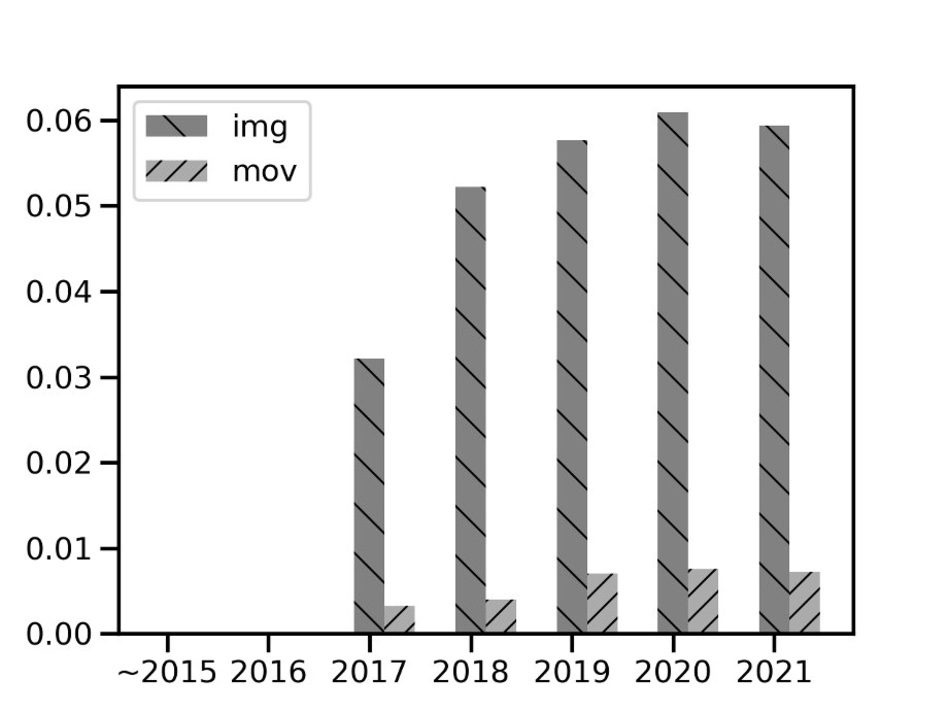
\includegraphics[width=1\linewidth]{./figures/data-category-trend.pdf}
\caption{ 
  An overview of the data collection
  }
\label{fig:data-collection-overview}
\end{figure*}


\subsection{Data Collection}
%\fig{fig:data-collection-overview} shows an overview of the data collection process. 
We first collected closed issue reports with \texttt{PyGitHub}\footnote{\url{https://pygithub.readthedocs.io/en/latest/index.html}} that internally execute GitHub API v3\footnote{\url{https://docs.github.com/en/rest}}. 
Next, we collected videos and images attached to the issue reports. While GitHub users can see videos and images on issue pages, the videos and images are stored in different URLs. As the URLs are written in the text description of issue reports, we parsed them with regular expressions and downloaded them. The regular expressions we used are shown as follows:
\begin{quote}
\addtolength\leftmargini{0in}
{\it https://user-images.githubusercontent.com/[a-zA-Z0-9\textbackslash-/]+\textbackslash.[a-zA-Z0-9]+}
\end{quote}
Each downloaded file was determined to be a image or video by its extension. Specifically, png, PNG, jpg, JPG, and jpeg are treated as images, and  gif, GIF, mp4, MP4, and mov as videos.
Consequently, we downloaded 33,079 images and 3,819 movies
with the collected URLs.\masa{to kuramoto: i wrote these numbers. are the numbers correct?} 


% \begin{table*}[h]
    \begin{center}
    \caption{Examples of the retrieved issues with the values of the attributes}
    \begin{tabular}{c c c c c c c} 
      \toprule
      \textbf{IssueCreatedYear} &
      \textbf{ResolutionTime} &
      \textbf{Images} &
      \textbf{Videos} &
      \textbf{Comments} &
      \textbf{FirstCommentTime} &
      \textbf{DescriptionLength} \\
      \midrule
      2020 & 6.99861111 & 0 & 0 & 1 & 6.99861111 & 4430\\
      2020 & 41.9594329 & 1 & 0 & 3 & 17.7784722 & 85\\
      2020 & 43.8850579 & 0 & 0 & 2 & 0.49828704 & 56\\
      2020 & 44.0935532 & 0 & 0 & 4 & 0.91277778 & 33\\
      2020 & 0.14934028 & 0 & 0 & 8 & 0.08077546 & 244\\
      2020 & 59.5670949 & 2 & 0 & 5 & 0.39472222 & 102\\
      2020 & 74.9322569 & 0 & 0 & 0 & -          & 24\\
      \bottomrule
    \end{tabular}
    \label{tab:example-dataset}
    \end{center}
  \end{table*}

% We extract a part of the retrieved issues in \tab{tab:example-dataset}. 
% Each row corresponds to the values of the attributes of an issue. 
%
\begin{table}[t]
    \begin{center}
    \caption{The attributes we collected from the issues}
    \scalebox{0.85}[0.85]{
    \begin{tabular}{ll} 
        \toprule
        \multicolumn{1}{c}{\textbf{Attributes}} & \multicolumn{1}{c}{\textbf{Description}} \\ 
        \midrule
        $IssueResolvedTime$ & The time until the issue is resolved (day) \\
        $FirstCommentTime$ & The time until the first comment (day) \\
        $\#comments$ & The number of comments \\
        $\#chars$ & \masa{im not sure what is this} \\
        $\#imgs$ & \# of attached images when the issue is created \\
        $\#movs$ & \# of attached movies when the issue is created \\
        $\#words$ &  \masa{im not sure what is this} \\
        $IssueCreatedYear$ & The year when the issue is created \\
        \bottomrule
    \end{tabular}
    }
    \label{tab:issue-attr}
    \end{center}
\end{table}


\begin{table}[t]
    \begin{center}
    \caption{The attributes we collected from the issues}
    \scalebox{0.85}[0.85]{
    \begin{tabular}{ll} 
        \toprule
        \multicolumn{1}{c}{\textbf{Attributes}} & \multicolumn{1}{c}{\textbf{Description}} \\ 
        \midrule
        $IssueResolvedTime$ & The time until the issue is resolved (day) \\
        $FirstCommentTime$ & The time until the first comment (day) \\
        $\#comments$ & The number of comments \\
        $\#chars$ & \masa{im not sure what is this} \\
        $\#imgs$ & \# of attached images when the issue is created \\
        $\#movs$ & \# of attached movies when the issue is created \\
        $\#words$ &  \masa{im not sure what is this} \\
        $IssueCreatedYear$ & The year when the issue is created \\
        \bottomrule
    \end{tabular}
    }
    \label{tab:issue-attr}
    \end{center}
\end{table}

\subsection{Analysis}
We retrieved the attributes from the collected issue reports.
\tab{tab:issue-attr} shows seven attributes extracted from 
the issue reports. 
The attributes can be classified into three dimensions, 
``Report'', ``Discussion'', and ``Fix''. 
The attributes in the dimension ``Report'' are extracted from 
the description of issue reports or attached files 
when the issue was created. 
In particular, in RQ1, we 
%calculate 
utilize the number of words 
in reports (\ie, $DescriptionLength$) for Img, Vid, and None. 
In addition,  $\#imgs$ and $\#vids$ are used to show 
dataset description. 
Note that these attributes are not calculated from either title, not comments (i.e., only descriptions were used). 
Also, when computing $DescriptionLength$, if the description of the issue report 
includes URLs for images/videos, 
we exclude them from the description because these are not words.

The dimension ``Discussion'' has two attributes, $Comments$ and $FirstCommentTime$. $Comments$ is the number of comments were made in the issue report. We utilize this attribute as a proxy measure of discussion effort. $FirstCommentTime$ is the days subtract from when the first comment was made to when issue was reported. We employ this attribute for measuring developers' interest. 

The dimension ``Fix'' has one attribute $IssueResolvedTime$ which shows the time from reported to fixed. 
Note that some negative values of $IssueResolvedTime$ were observed. We investigated it manually and found that these are because of a bug in GitHub.  We excluded those issues that have negative values from our dataset. 
In addition, we excluded issue reports resolved in too short or long periods (e.g., 30 seconds) because they might be issued after being fixed or might not be fixed in reality.
%\kashiwa{check please}
Specifically, we only use the issue reports that meet the condition: $30\ sec \leq IssueResolvedTime \leq 1\ year$.
The number of issue reports that meet this condition is 711,160 (92.23\%).


\kashiwa{Write what do you analyze (e.g., compare them in median)}
To evaluate the difference, we used a non-parametric test \textit{Steel-Dwass test}.
\kashiwa{Write what this test is}
\kashiwa{Write why this test is selected}
because our preliminary study shows that 
the distributions for each category do not 
come from normal distributions.
\kashiwa{Write the reason why correction is not needed (i.e., how to deal with family-wise error rate)}






% We used $Words$ to compute the TFIDF values\masa{need citation} for each category. 
% The TFIDF values will support researchers who investigate 
% the differences in the appearances of words with and without 
% images/movies. 
%% We suppose that images and movies are utilized to 
%% describe specific contents such as GUI bugs. 
%% Hence, we computed the TFIDF values\masa{need citation} 
%% on $Words$ for each category. 
%% The TFIDF values clarify the differences in the appearances of 
%% words with and without images/movies. 

\newpage
\subsection{Data Description}

\begin{table}[h]
    \begin{center}
    \caption{The number of issues for each category}
    \begin{tabular}{llr}
        \toprule
         & \multicolumn{1}{c}{\textbf{Description}} & \multicolumn{1}{c}{\textbf{\#issues}} \\
        \midrule
        $Img$  & $\#imgs \geq 1$ & 33,079 (4.65\%)\\
        $Mov$  & $\#movs \geq 1$ & 3,819 (0.54\%)\\
        $None$ & Others & 674,793 (94.81\%)\\ 
        \bottomrule
    \end{tabular}
    \label{classify_result}
    \end{center}
\end{table}

We classified the collected issue reports into three categories based on whether they have images and movies. \tab{tab:issue-category} shows the number of issue reports for each category. 
Note that issue reports often have both images and movies. 
These issue reports are counted in both $Img$ and $Mov$ categories (only X\%). 
Thus, the total number of downloaded issue reports is different from the sum of \#issues in \masa{Table X}\masa{Kashiwa-sensei wrote this right? I highlight the unknown table number->Yes}. 
In this paper, we refer to the issue reports in the $Mov$ category 
as \textit{visual issue reports}. 

\begin{figure}[h]
\centering
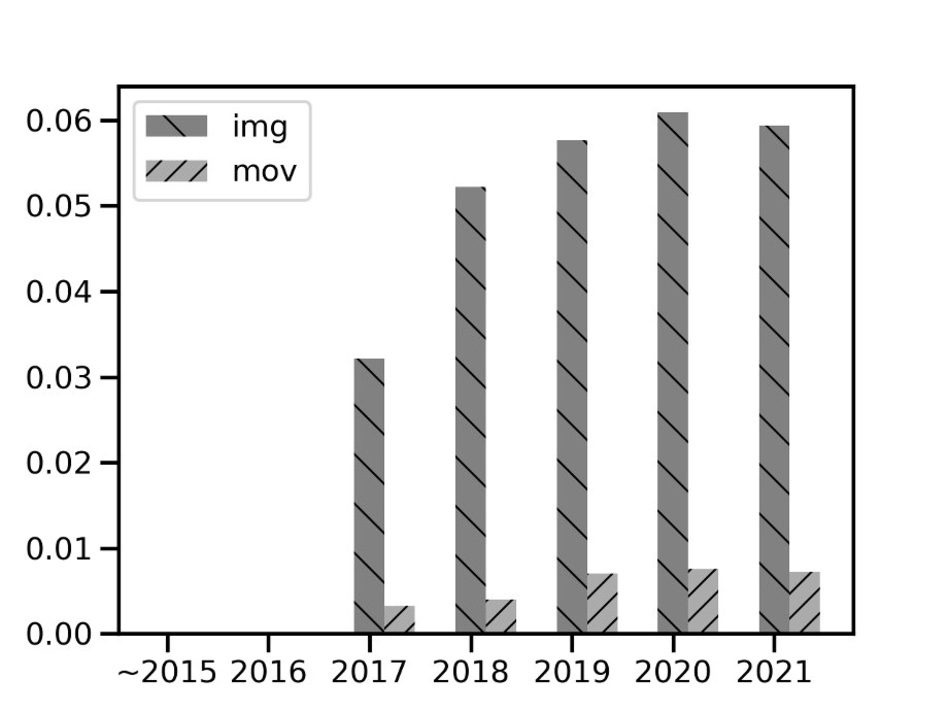
\includegraphics[width=0.6\linewidth]{./figures/data-category-trend.pdf}
\caption{ 
  The proportions of issue reports for each category
  }
\label{fig:data-cat-trend}
\end{figure}
We collected XXX videos and XXX images from XXX issue reports. Out of the collected issues, only 4.65\% of issue reports have images, and 0.54\% have videos. While this number seems to be small, looking into the trend shown in \fig{fig:data-cat-trend}, the rate of visual issue reports by year is increasing from 2017 to 2020. The ratio of visual issue reports reached to 5\% between 2018 and 2021.


\section{Results}
\label{sec:results}

% 初期段階の調査として,画像及び動画がissueの各attributesに
% 与える影響について調査する.
% 表2で得られたそれぞれのカテゴリ間で比較を比較を行う.
% 等分散性を仮定できないデータが含まれていたため,
% 比較にはSteel-Dwass testを採用する.
% 
% visualizationは,issueの解決時間,
% コメント数,文字数に何らかの影響を与える.
% 検定結果を表6に示す.
% 有意水準は0.05を採用する.
% IssueResolvedTimeにおいて,
% ImgとMovは片側検定で有意差があった.
% また,表Xより,平均値,中央値でNoneカテゴリの
% issueよりImgとMovカテゴリのissueの方が
% 課題解決時間が長かった.
% よって,画像もしくは動画がissue作成時に付与
% される課題はその解決時間が有意に長くなる.
% また,#comments及び#charsでは両側検定で
% 有意であり,これらのattributesにも
% 有意な影響を与えることがわかった.
% ただし,imageとmovieに有意差は
% 観測されなかった.

% As an initial analysis, we investigated 
% the impact of images and movies on 
% the issues in terms of the attributes. 
% As an initial analysis, 


\subsection*{RQ1: \RQone{}}
\begin{figure}[t]
    \centering
    %\includegraphics[width=0.5\linewidth]{tex-kondo/figures/words.png}
    \includegraphics[width=0.5\linewidth]{./figures/words.png}
    %\caption{Distributions of words written in issue reports. }
    %\caption{Boxplots of \# of words written in the description }
    \caption{The attribute in the Report dimension}
    \label{fig:words}
\end{figure}
%\textbf{DescriptionLength of visual issue reports is 
%similar to the others.}

\fig{fig:words} shows the distributions in the number of words 
written in descriptions of issue reports. 
%The green line in the box shows the median, 
%the bottom and the top lines of the box show 25 and 75 percentile, respectively. 
The median of DescriptionLength was 36 words in Img, 
46 in Vid, and 36 in None. 
The number of words in videos is slightly larger than 
the others but no statistically significant differences are observed. 
This implies that reporters write as many texts as the others 
to describe the contents of videos. 

\summarybox
%{Answer to RQ1}
{{\bf RQ1: }{No, visual issue reports still require reporters 
to write similar amounts of texts to describe bugs. 
}}

\subsection*{RQ2: \RQtwo{}}
\begin{figure}[t]
    \centering
    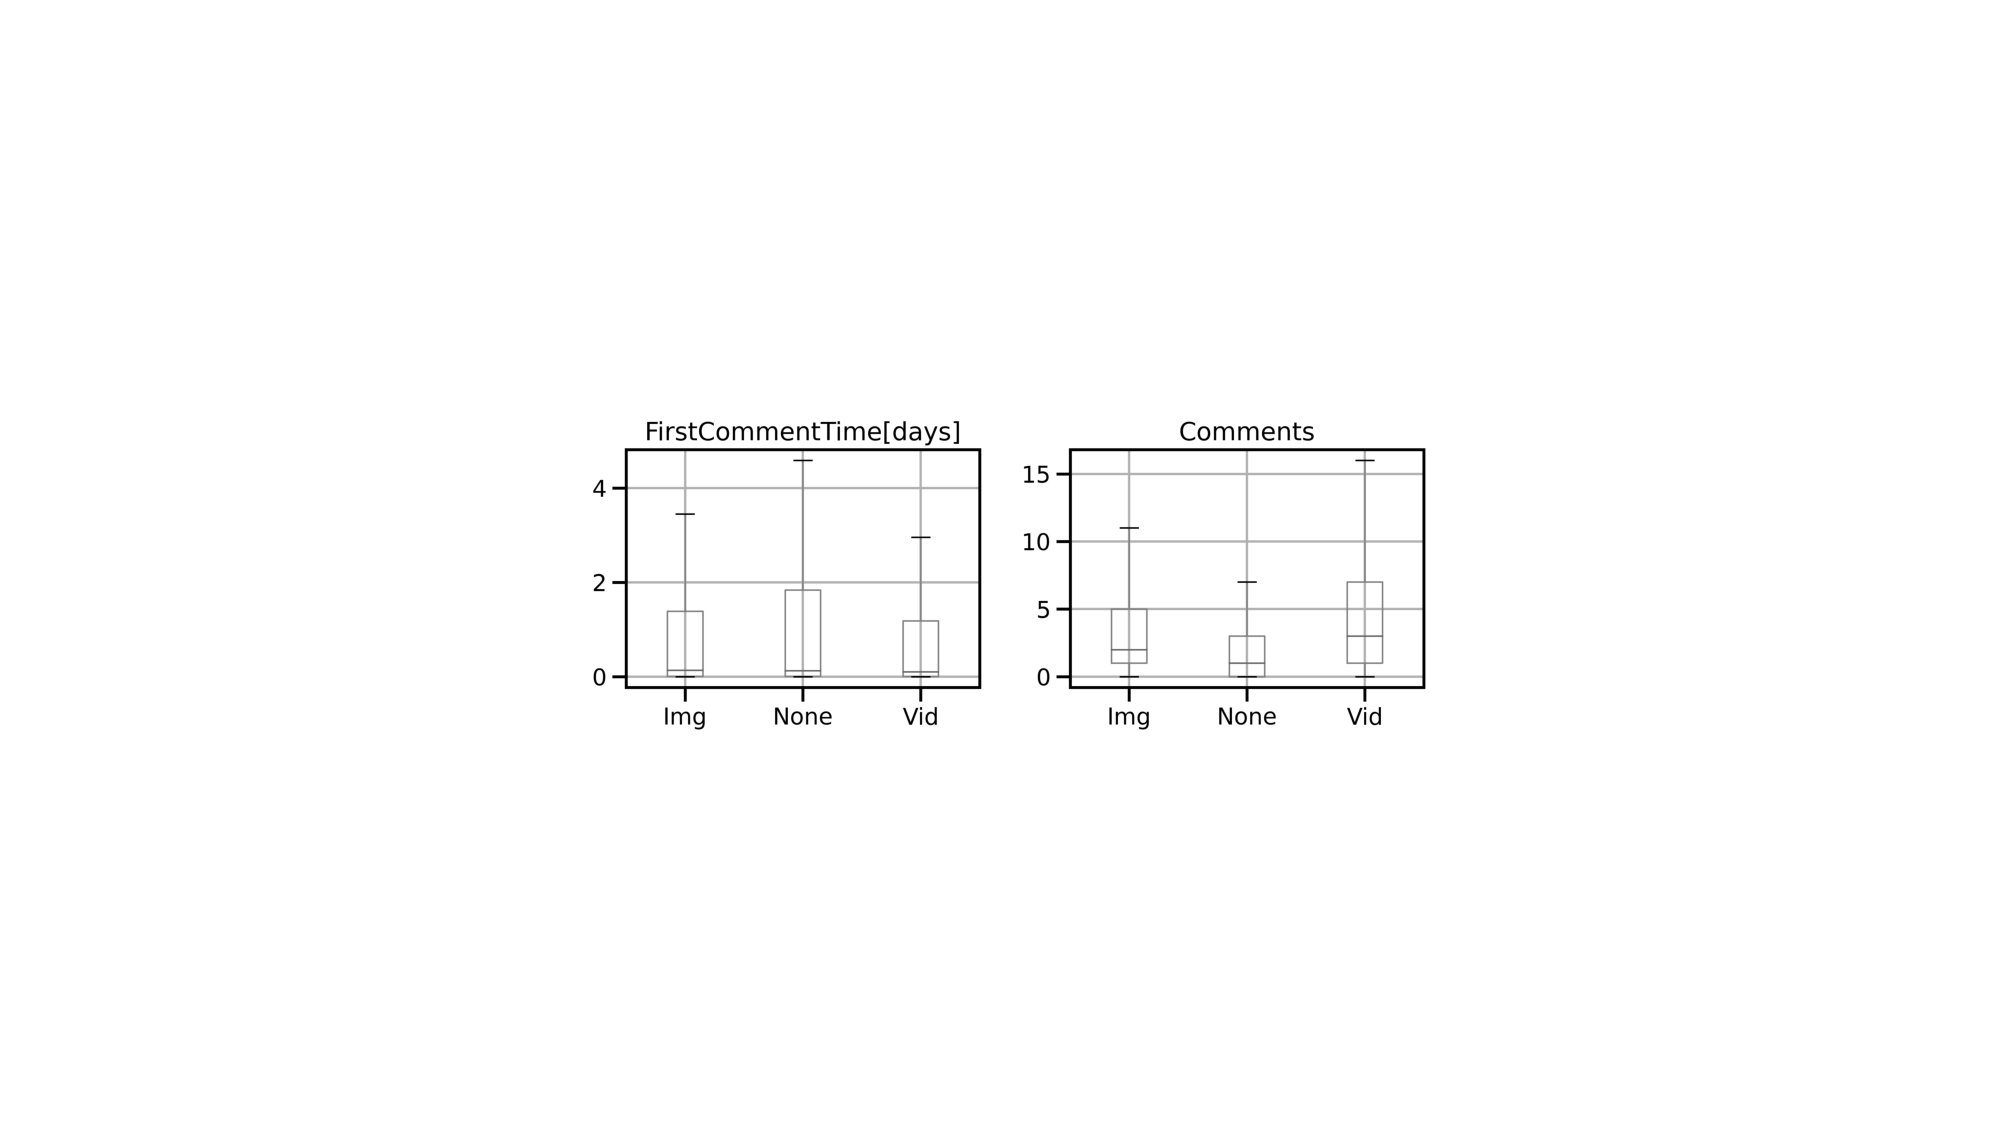
\includegraphics[width=1\linewidth]{./figures/discussions.pdf}
    %\caption{Amount of texts written in issue reports. }
    \caption{The attributes in the Discussion dimension}
    \label{fig:discussion}
\end{figure}


\fig{fig:discussion}
shows the values of the Discussion dimension
for each category. 
We observed that the 25th, 50th, and 75th percentiles of 
the $Vid$ category in 
this dimension
%$FirstCommentTime$ and $\#comments$ 
result in the largest or faster values than those of 
the other two categories.
Hence, the visual issue reports get more responses 
while they get faster responses. 
%% 
%% 
%% %However, we do not observe significant differences 
%% \textbf{
%% However, we occasionally observe non-significant differences
%% in $FirstCommentTime$ and $\#comments$.}
%% %\textbf{
%% %However, the visual issue reports are not significantly different 
%% %from the issue reports in the Img category
%% %in $FirstCommentTime$ and $\#comments$.
%% %}
%% \tab{tab:Steel-Dwass-test} shows the results of 
%% the Steel-Dwass test. 
%% 
%% The asterisks indicate significance based on 
%% the Steel-Dwass test: * indicates $p$ < 0.05 in 
%% the two-sided test; 
%% ** indicates $p$ < 0.05 in the one-sided test. 
%In summary, the visual issue reports do not show 
%significant differences compared with 
%the issue reports with images in 
%In summary, the visual issue reports are not 
%significantly different from the issue reports 
%in the Img category, 
%whereas visual issue reports and 
%the issue reports in the Img category 
%are significantly different from the issue reports 
%in the None category in
%$FirstCommentTime$ and $\#comments$.
%In summary, the visual issue reports are not 
However, the visual issue reports are not 
significantly different in $FirstCommentTime$ 
compared with the other two categories and 
are not significantly different in $Comments$ 
compared with the Img category.

\summarybox
%{Summary of RQ2}
{{\bf RQ2: }{Yes, more active discussions happen in visual issue reports. Visual issue reports are 3-times likely to receive more comments than reports without images or videos. }
}









\subsection*{RQ3: \RQthree{}}
\begin{figure}[t]
    \centering
    %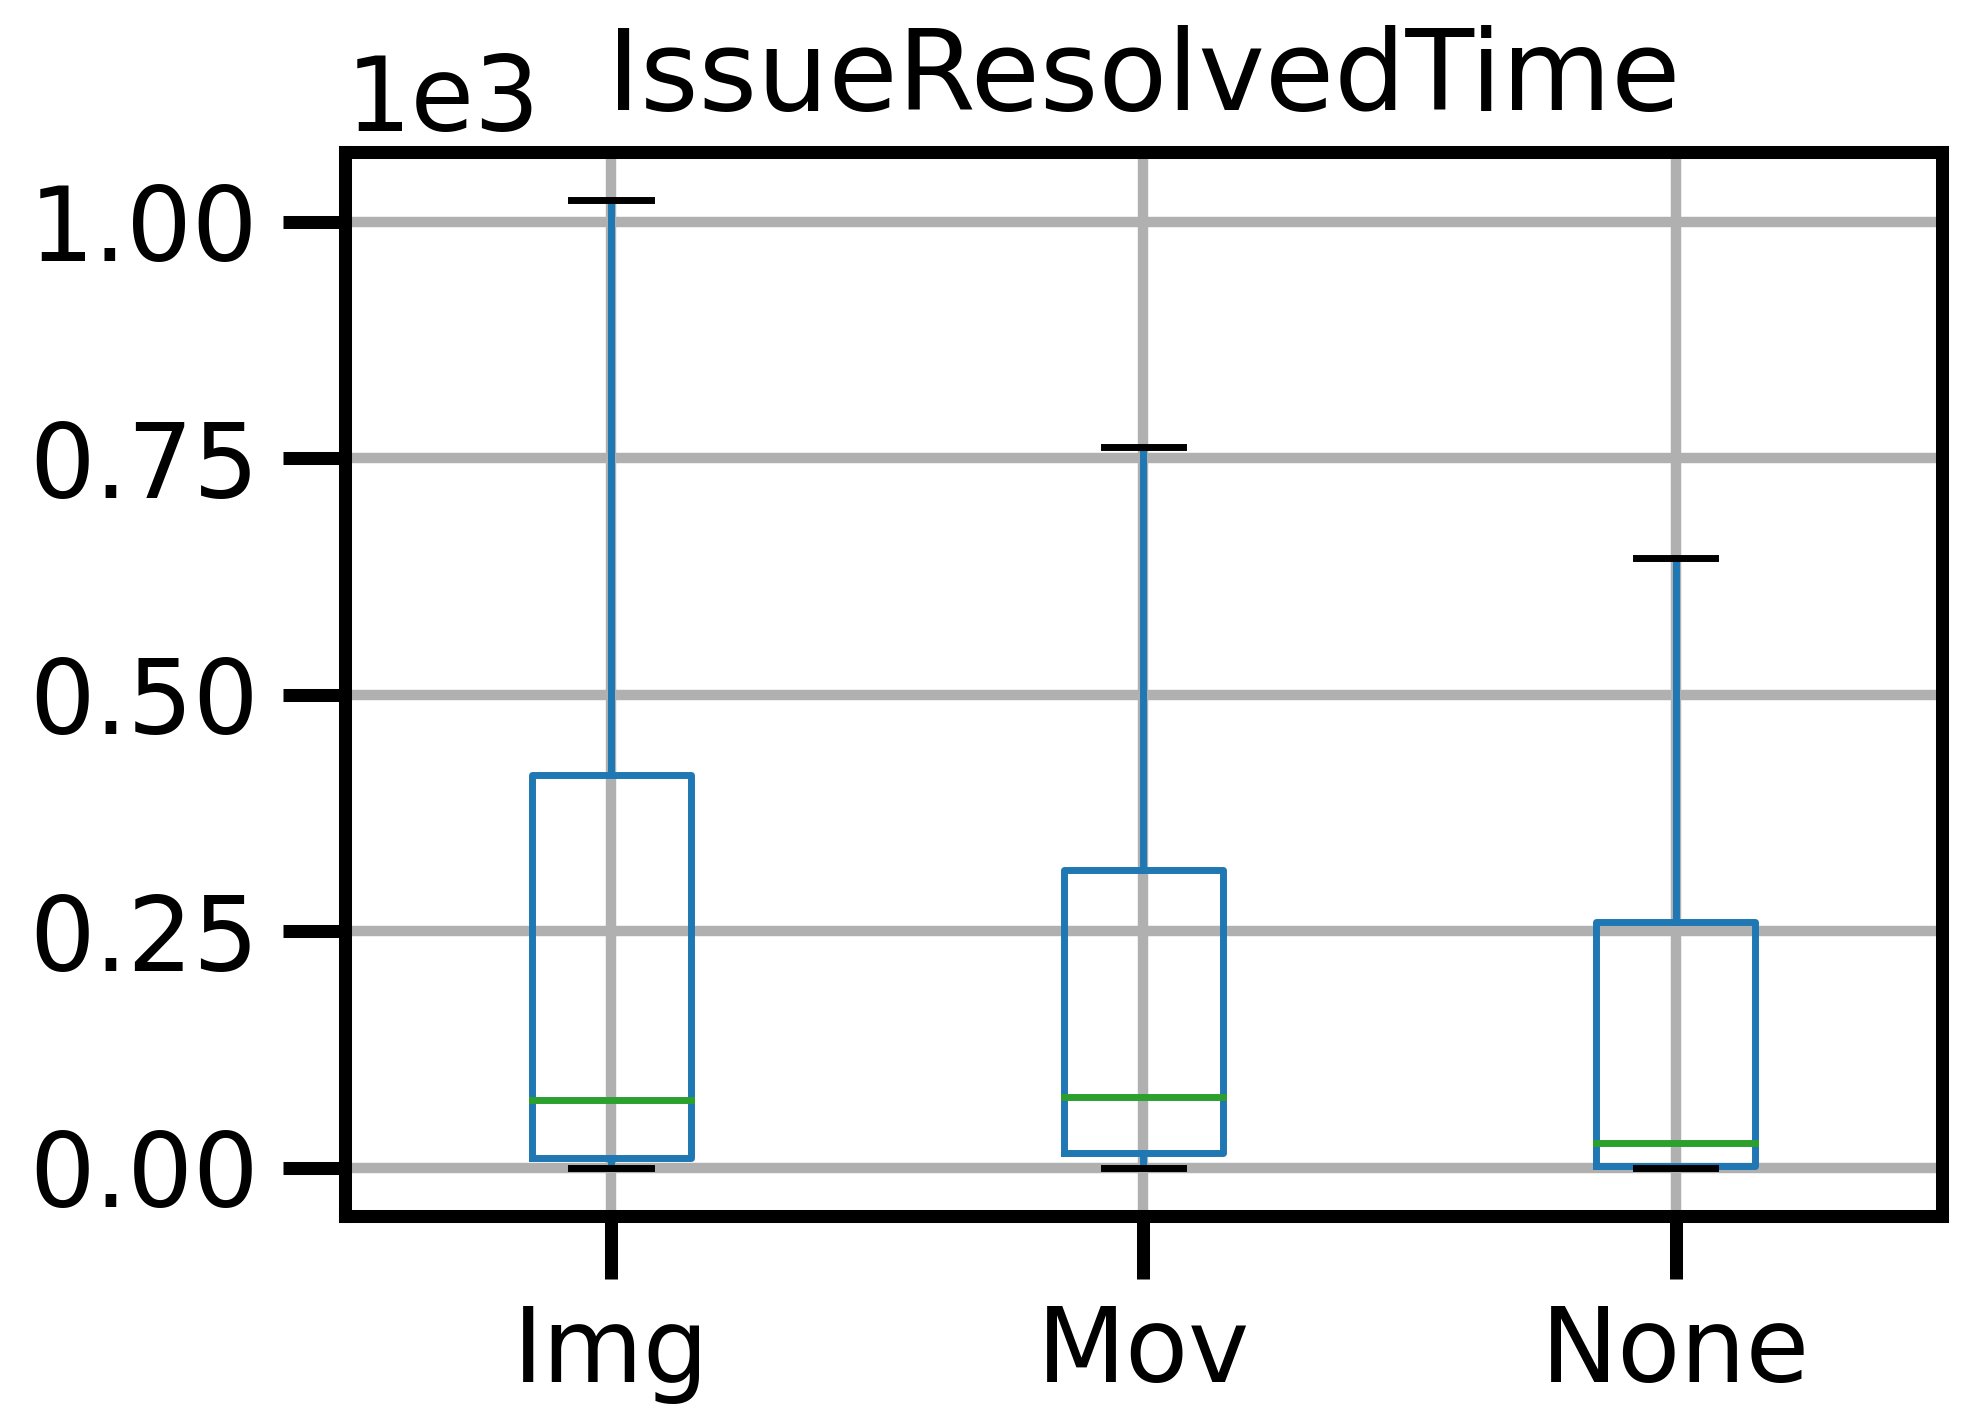
\includegraphics[width=0.6\linewidth]{tex-kondo/figures/fixes.png}
    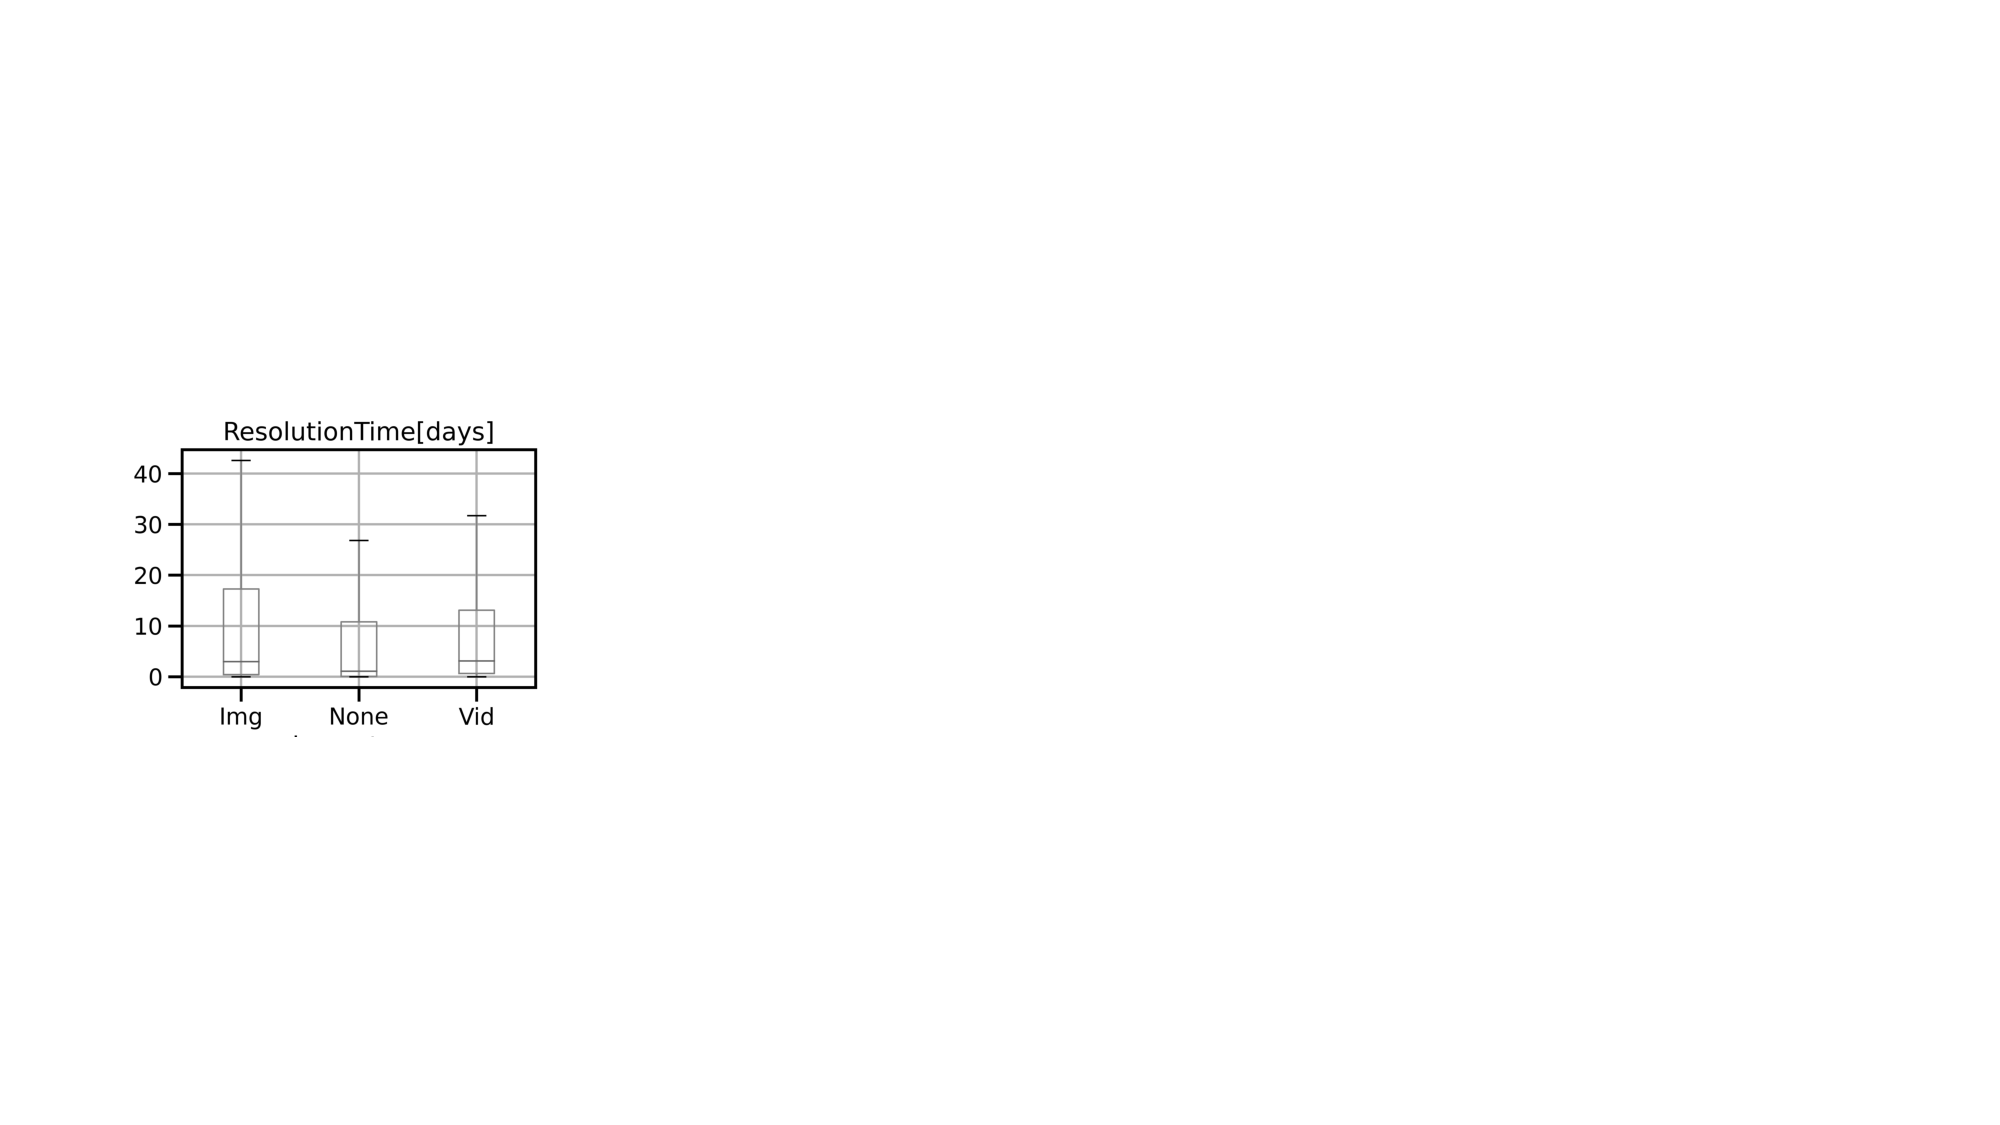
\includegraphics[width=0.5\linewidth]{./figures/fixes.pdf}
    %\caption{Amount of texts written in issue reports. 
    %The median of \#word was 2.96 in Img, 3.01 in Vid, and 1.09 in None.
    %\masa{I moved this comment to here (maybe removed later? I'm not sure)}
    %}
    \caption{The attribute in the Fix dimension}
    \label{fig:resolvedtime}
\end{figure}
%% We investigated 
%% the differences with and without images and movies 
%% for each attribute on the issues. 
%% Specifically, we compared the attributes between 
%% the categories in \tab{tab:issue-category}. 
%% Because our preliminary study shows that 
%% the distributions for each category do not 
%% come from normal distributions, 
%% we used a non-parametric test called the \textit{Steel-Dwass test}. 


%% %\textbf{The visual issue reports get resolved faster than 
%% \textbf{The visual issue reports need a longer time to be resolved than
%% the issue reports in the None category. }
%% % \textbf{The attribute values are changed 
% with and without images and movies.}
% \tab{tab:Steel-Dwass-test} shows the results of 
% the Steel-Dwass test. 
% The asterisks indicate significance based on 
% the Steel-Dwass test: * indicates $p$ < 0.05 in 
% the two-sided test; 
% ** indicates $p$ < 0.05 in the one-sided test. 
Contrary to our hypothesis, \fig{fig:resolvedtime} and our observation show that 
the mean and the median $IssueResolvedTime$ values of 
the issue reports in the $Img$ category and the $Vid$ category are 
longer than those in the $None$ category. 
Also, we observed that the issues in the $Img$ category and 
the $Vid$ category are significantly different from those 
in the $None$ category in terms of $IssueResolvedTime$.
%(\tab{tab:Steel-Dwass-test}). 
% \tab{tab:issue_stat_categories} shows the statistics
% of the collected issues for the $Img$, $Mov$,
% and $None$ categories.
% The Mean row indicates the average values; 
% the Min and Max rows indicate the minimum and maximum values; 
% the 25th, 50th, and 75th rows indicate the percentile values; 
% the S.D. row indicates the standard deviation values. 
% % We may not find the general conclusion; 
% % however, we observed differences across the categories. 
% % For example, the 25th, 50th, and 75th percentiles of 
% % the $Img$ and $Mov$ categories in $IssueResolvedTime$ are 
% % longer than those of the $None$ category. 
% % % \tab{tab:issue_stat_categories} shows that 
%This table shows that 
Hence, the issue reports with images or videos tend to need 
a longer time to be resolved. 

% In addition, we observed that the issues in 
% the $Img$ category and the $Mov$ category are 
% significantly different from those in 
% the $None$ category in terms of $\#comments$ and 
% $\#chars$. 
% Hence, the issues with images or movies 
% tend to have different numbers of 
% comments and words in the issue description.

% It should be noted that we do not observe 
% the difference between the $Img$ category and 
% the $Mov$ category. 


%{\bf No, resolution time for issues with videos are not different from those for the others. 
\summarybox
%{Summary of RQ3}
{{\bf RQ3: }{No, resolution time of visual issue reports is longer than that of other issue reports.
}}





\section{Future Research Plan}
\label{sec:future}



% \section{Limitation}
\subsection{Threats to Validity}
\label{sec:limitation}

While the number of issue reports that we studied is 770,656,  this number accounts for only less than 2\% of all the repository due to the time limitation. 
We believe that the selection of repositories is not biased because we randomly selected these repositories. 
Still, we cannot generalizerize the findings in this study. 

In addition, since GitHub released the feature to post videos in May 2021, this feature is still new and yet to be common. The number of visual issue reports has increased as \fig{fig:data-cat-trend} shows, and then the results may vary after the feature becomes popular. 

We collected the issue reports with PyGitHub. 
However, in this process, some pull requests were also collected due to the specification of GitHub. 
Hence, our analysis may include such pull requests as issue reports. \kashiwa{RECHECK}
\section{Related Work}
\label{sec:relate}
While numerous studies have worked on bug resolution time~\citep{DBLP:conf/msr/ChenNSH14}\citep{DBLP:journals/jss/GarciaSN18}\citep{DBLP:conf/sigsoft/JeongKZ09}\\
\citep{DBLP:conf/icsm/KashiwaYKO14}\citep{DBLP:conf/msr/ZamanAH11}, 
in particular, the following studies investigated the relationship between bug resolution time and various elements of bug reports other than videos~\citep{DBLP:conf/msr/BhattacharyaN11}\citep{DBLP:conf/csmr/BhattacharyaUNK13}\citep{DBLP:journals/ieicetd/NoyoriWFKONT21}. 
Noyori~\et~\citep{DBLP:journals/ieicetd/NoyoriWFKONT21} investigated the relationship between resolution time and topics included in the comments of issue reports. 
They found that bugs are resolved fast when discussions about symptoms are not needed.  Bhattacharya \et \citep{DBLP:conf/msr/BhattacharyaN11} developed bug-fix
time prediction models using various metrics. They showed that bug severity and the number of attachments (patches) do not correlate with bug-fix time. In addition, their later work by Bhattacharya \et~\citep{DBLP:conf/csmr/BhattacharyaUNK13} compared bug-fix time for high-quality and poor-quality reports. They observed that the text length of descriptions is relatively correlated with bug resolution time. 

A few recent studies have utilized visual issue reports for improving bug-fixing process~\citep{DBLP:conf/icse/CooperBCMP21}. Cooper~\et~\citep{DBLP:conf/icse/CooperBCMP21} used videos and texts included in issue reports to detect duplicate issue reports. Compared with the study, the contribution of our work is (1) the analysis of the impact of visual issue reports and (2) the public available datasets consisting of 1,324 videos and 21,003 images from 241,398 issue reports.
\section{Conclusion}
\label{sec:conclusion}

\masa{conclusion here}

Finally, we present future research directions with our dataset. 


\noindent
\textbf{The impact analysis of movies and images on software development.}
GitHub added the feature~\citep{github-video-blog} to easily 
share movies with GitHub to earn advantages 
in software development such as reproducing bugs easily in issues and 
explaining the background of changes in pull requests. 
However, no studies exist that investigate whether such movies 
impact software development. 
Hence, investigating the impact of movies on software development 
is a future research direction. 
Specifically, we study the reduction of issue resolution time, 
the response rate of developers, and 
the reduction of the number of comments 
in which developers write ``works for me''. 

\noindent
\textbf{Automated bug reproduction with image processing.}
Reproducing bugs is a time-consuming process 
in software development\masa{citation}.
Automating this process would support developers 
to quickly find and fix the cause of bugs. 
Hence, it is an important future research direction 
to automate bug reproduction. 
As the evolution of image processing with deep learning models, 
the accuracy of image processing significantly improves\masa{citation}. 
Hence, we apply such deep learning models to movies 
to implement automated bug reproduction tools. 


\section*{Acknowledgment}
This work has been supported by JSPS KAKENHI Japan
(Grant Numbers: \masa{update}.


\bibliographystyle{ACM-Reference-Format}
\bibliography{reference}



\end{document} 
